\section*{TA Questions \pts{0}}

This section is for TAs to put their draft questions into. Please see the qtemplates.tex file for how to format the questions. 


\begin{questions}

\question[5] \textit{Feature Engineering.} Consider the following 1-D dataset.
\\ 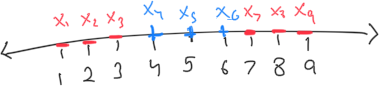
\includegraphics[width=6cm,height=2cm]{figures/FE_1D.png}
    \noaddpoints % to omit double points count
    \begin{parts}
    \part[3]  \textbf{Short answer:} Engineer a second feature such that the data set becomes linearly separable in 2 dimensions. i.e, if the two new features are $x_1' = x$ and $x_2'=f(x)$, give an expression for f.
    \fillwithlines{2em}
    \begin{soln}
    Many answers possible
    $f(x)= (x-5)^2$,  $f(x)= |x-5|$\\
    Brynn's comment: I like this question, but it could be quite difficult to grade. If we want to simplify grading, we could do a select all that apply or select one with many options. But there is something learned having them write this themselves that I kind of like. The image should be fixed.  \\ Tom's comment: I agree this is a good question, but it'll be too difficult to ask students to submit drawings on this remote exam.  I suggest including this question but reworded as a "check all that apply" question as Brynn suggests. Then drop part B.
    \end{soln}
    \part[2] \textbf{Short answer:} Draw the transformed 2-dimensional Dataset along with a linear hyperplane that perfectly separates the data.
    \begin{soln}
    \\\includegraphics[width=5cm,height=5cm]{figures/FE_Solution.png}
    
    Brynn's comment: So far, we have not had students submit drawings. Is this something we want to try? If not, we would need a description, which would again make this hard to grade. Parts a and b would need to be graded together. 
    \end{soln}
    \end{parts}
    \addpoints
    \begin{qauthor}
    Input (1)Varun Natu, (2) Feature Engineering and creating linearly separable data by moving to higher dimensions
    \end{qauthor}
    
    
\question[3] Consider the following flattened representation of a convolution layer over a 3x3 image with the connections missing.
    \\ 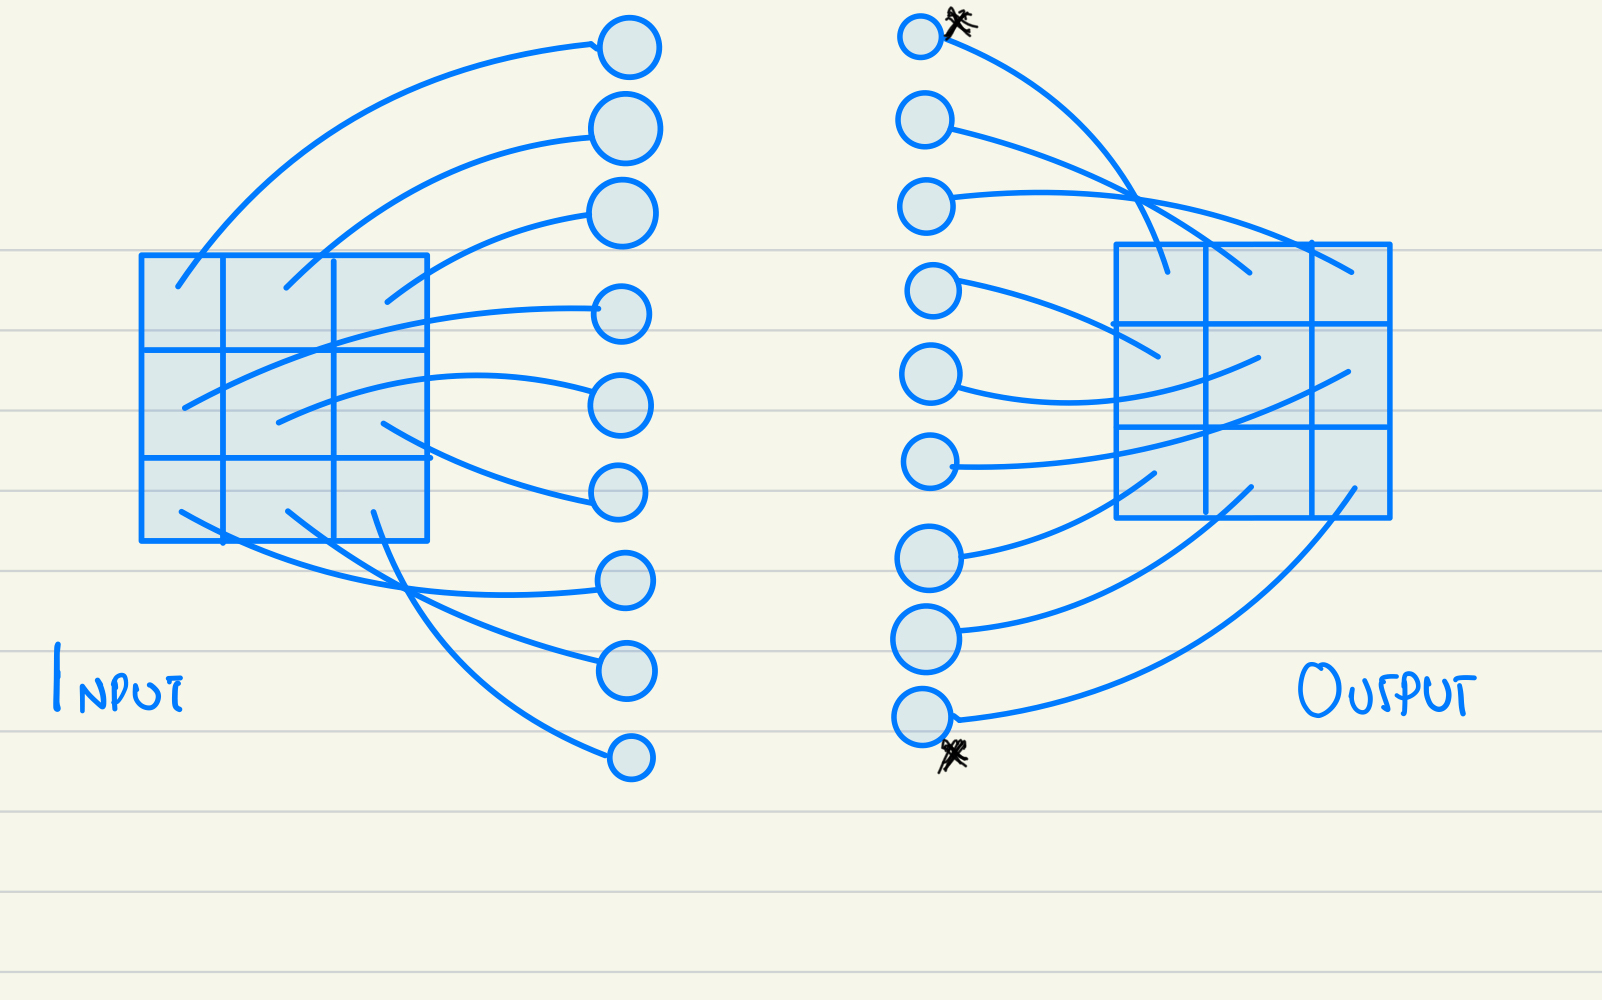
\includegraphics[width=4cm,height=4cm]{figures/CNN_flat.jpeg}

    \textbf{Short answer:} Draw the appropriate connections for the output cells with an asterix next to them and mark each edge with the corresponding kernel weight.
    \begin{soln}
    \\\includegraphics[width=6cm,height=6cm]{figures/CNN_Solution.jpeg}\\
    Brynn's comment: I don't see how we can do this as students would have to re-draw the image. I think this question is better suited for an in person exam. I would probably cut this
    \end{soln}
    \begin{qauthor}
    Input (1)Varun Natu, (2) CNNs and parameter sharing
    \end{qauthor}
    
\question[1] \textbf{Multiple choice:} In which of the following environments would you expect deep Q-Learning to perform best?
    {%
    \checkboxchar{$\Box$} % change checkbox style locally
    \begin{checkboxes}
     \choice An environment with frequent rewards and low exploration cost. eg[Atari Brick-Breaker]  
     \choice An environment with sparse rewards and low exploration cost. eg.[A video game that gives reward only on completing a full level]
     \choice An environment with sparse rewards and high exploration cost 
     \choice Q-learning can work equally well in all environments
    \end{checkboxes}
    }
    \begin{soln}
    A\\
    
    Brynn's Comment: I think this is fine, but I cannot remember how much this was discussed in class. Matt should review. \\ Tom Comment: I reworded this to ask which it will work "best" in, as I felt asking which it would work "well" in was a bit ambiguous.  I think we should include this if Matt approves. \\ Matt's comment: Good question, but I think we should have had something like it in homework / practice questions before including it on an exam. So let's move it to practice questions.
    \end{soln}
    \begin{qauthor}
    Input (1) Varun Natu (2) Limitation of deep Q-learning and dependence on frequent rewards and environment exploration
    \end{qauthor}
\question[1] \textbf{Select all that apply:} Which of the following algorithms are capable of learning the decision boundary drawn in yellow ?
\\ 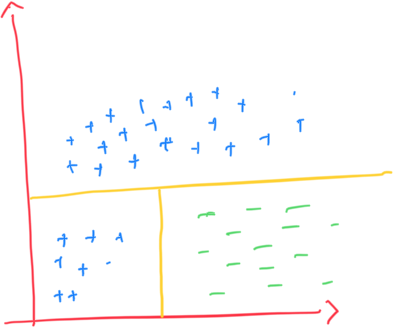
\includegraphics[width=5cm,height=5cm]{figures/decision_boundaries.png}
    {%
    \checkboxchar{$\Box$} % change checkbox style locally
    \begin{checkboxes}
     \choice Logistic Regression 
     \choice Linear Regression
     \choice Decision Tree
     \choice KNN
     \choice Neural Network
    \end{checkboxes}
    }
    \begin{soln}
    C,E\\
    Brynn's comment: I like this question. Would a NN definitely find a bound this smooth? \\ Tom comment: good quesiton, yes the right neural net can approximate this boundary arbitrarily well.
    \end{soln}
    \begin{qauthor}
    Input (1) Varun Natu (2) Linear + Non-linear decision boundaries 
    \end{qauthor}


\question[1] \textbf{Select one:} Assume there are three output classes instead of binary classes for logistic regression. Is it possible to extend binary logistic regression to classify three unique discrete classes? Why or why not? (p is the output of the sigmoid function)
    \begin{checkboxes}
     \choice Yes, train three different binary logistic regression models that classify one class from the other two
     \choice Yes, divide sigmoid function into three cutoffs, where first class will be assigned to $p < \frac{1}{3}$, second class to $\frac{1}{3} \leq p < \frac{2}{3}$, and third class to  $\frac{2}{3} \leq p$
     \choice No it is not possible
    \end{checkboxes}
    \begin{soln}
    A\\
    
    Brynn's Comment: If we say we saw this in class doesn't it make it obvious the answer is yes? This may be a better short/open ended question just asking them if this is possible and if so/not to describe why as discussed in class.  \\ Matt's comment I wasn't sure from the question whether we were fishing for a reduction to multiclass or multilabel classification, maybe clarify.
    \end{soln}
    \begin{qauthor}
    (1) Daniel Min (2) Application of binary logistic regression into multinomial logistic regression
   
    \end{qauthor}


\question[1] \textbf{True or False:} The fixed point method will find the optimal solution to an optimization, as long as the function is convex.
    \begin{checkboxes}
     \choice True 
     \choice False
    \end{checkboxes}
    \begin{soln}
    False, the function must be a contraction mapping over the domain of interest in order for the Banach fixed point theorem to apply.
    \end{soln}
    \begin{qauthor}
    Input (1) Everett Knag (2) Value iteration theoretical understanding \\
    Matt's comments: Great question -- I should have mentioned this in class, but didn't. So not including it for now.
    \end{qauthor}

\end{questions}